\chapter{Perancangan Sistem}

\section{Analisis Kebutuhan Sistem}

Analisis kebutuhan sistem dilakukan untuk mengidentifikasi kebutuhan fungsional dan non fungsional
pada platform manajemen aset, inventori, dan rental berbasis web yang dikembangkan dalam proyek
\textit{capstone}. Tahap analisis kebutuhan dilakukan sebagai dasar dalam perancangan arsitektur
multitenant agar sistem mampu mendukung pengelolaan banyak organisasi dalam satu platform secara
efisien dan terpusat.

Pada platform \textit{multi organization}, setiap organisasi memiliki pengguna, data, serta proses
operasional yang berbeda sehingga sistem memerlukan mekanisme pengelolaan tenant yang mampu
menjaga isolasi data antar organisasi. Selain itu, sistem juga memerlukan mekanisme
\textit{provisioning} tenant yang mendukung proses \textit{onboarding} tenant baru secara lebih
cepat dan konsisten tanpa meningkatkan kompleksitas pengelolaan sistem.

Berdasarkan kebutuhan tersebut, analisis dilakukan terhadap kebutuhan pengelolaan tenant,
kebutuhan isolasi data, kebutuhan \textit{scalability} sistem, serta efisiensi penggunaan
\textit{resource} infrastruktur pada platform \textit{multi organization}. Hasil analisis
kebutuhan ini digunakan sebagai dasar dalam perancangan arsitektur multitenant berbasis
\textit{shared database} dan \textit{shared schema}.

\section{Gambaran Umum Sistem}

Sistem yang dikembangkan merupakan platform manajemen aset, inventori, dan rental berbasis web
yang dirancang untuk mendukung banyak organisasi dalam satu layanan terpusat. Platform ini
memungkinkan setiap organisasi memiliki pengguna, data, dan proses operasional masing-masing
dalam satu aplikasi bersama.

Dalam implementasinya, setiap tenant memiliki kebutuhan pengelolaan data yang terpisah sehingga
sistem memerlukan mekanisme isolasi data untuk memastikan setiap organisasi hanya dapat mengakses
data miliknya sendiri. Selain itu, sistem juga memerlukan mekanisme pengelolaan tenant yang mampu
mendukung \textit{onboarding} tenant baru secara efisien tanpa memerlukan konfigurasi infrastruktur
yang terpisah untuk setiap organisasi.

Untuk mendukung kebutuhan tersebut, sistem dirancang menggunakan pendekatan arsitektur multitenant
berbasis \textit{shared database} dan \textit{shared schema}. Pendekatan ini memungkinkan seluruh
tenant menggunakan aplikasi dan basis data yang sama dengan tetap mempertahankan isolasi data antar
tenant melalui mekanisme \textit{tenant scoping} pada \textit{application layer}.

Pada sistem yang dirancang, pengguna akan melakukan autentikasi ke dalam platform dan setiap proses
akses data akan disesuaikan dengan konteks tenant pengguna yang sedang \textit{login}. Dengan
pendekatan tersebut, platform dapat mendukung pengelolaan banyak tenant secara lebih efisien,
terpusat, dan \textit{scalable} dibandingkan pendekatan non multitenant yang menggunakan
\textit{instance} terpisah untuk setiap organisasi.

Ruang lingkup sistem dalam penelitian ini mencakup pengelolaan data aset, inventori, dan rental
sebagai konteks penerapan arsitektur multitenant. Sistem dirancang untuk mendukung penggunaan oleh
banyak tenant dalam satu platform, dengan mekanisme isolasi data, pengelolaan konteks tenant, dan
\textit{provisioning} tenant otomatis. Penelitian ini tidak mencakup pengembangan antarmuka
pengguna secara detail maupun optimalisasi performa tingkat rendah, melainkan berfokus pada
rancangan arsitektur dan mekanisme pendukung yang memastikan efisiensi infrastruktur dan keamanan
data pada platform multi organisasi.

\begin{figure}[h]
  \centering
  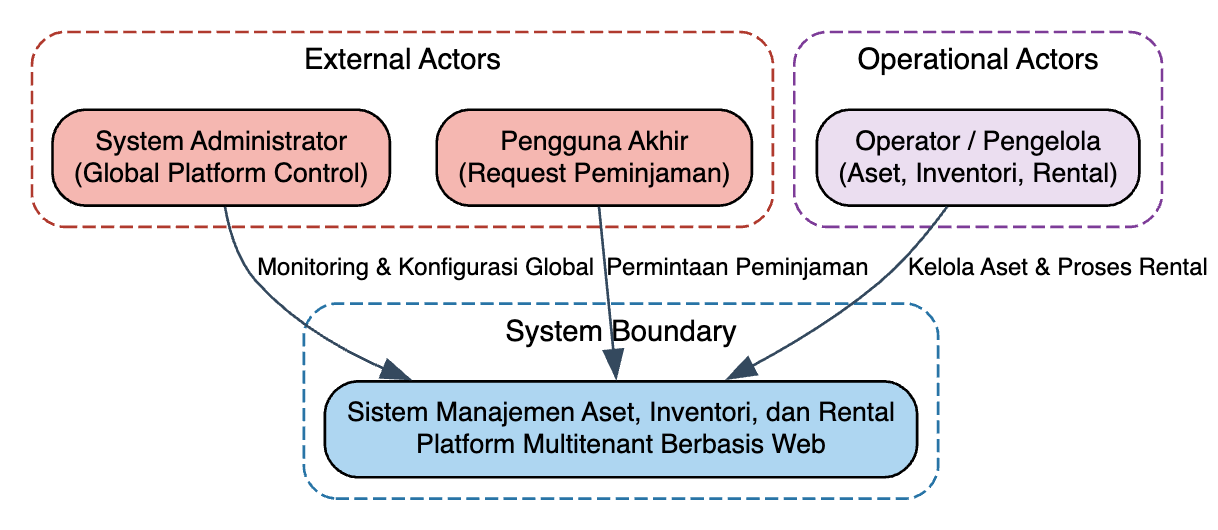
\includegraphics[width=0.9\textwidth]{assets/image2.png}
  \caption{Diagram Konteks Sistem Manajemen Aset, Inventori, dan Rental}
  \label{fig:diagram_konteks}
\end{figure}

\section{Perancangan Arsitektur Multitenant}

Perancangan arsitektur multitenant merupakan inti dari penelitian ini karena berfungsi sebagai
solusi terhadap permasalahan efisiensi infrastruktur dan pengelolaan data multi organisasi dalam
satu platform terpusat. Arsitektur yang dirancang harus mampu melayani banyak tenant secara
bersamaan tanpa mencampurkan data antar tenant, serta tetap efisien dari sisi penggunaan sumber
daya sistem.

\subsection{Pemilihan Arsitektur Multitenant}

Arsitektur yang dipilih dalam penelitian ini adalah arsitektur multitenant berbasis aplikasi
terpusat, di mana satu \textit{instance} aplikasi digunakan oleh seluruh tenant. Setiap permintaan
yang masuk ke sistem diproses dalam konteks tenant tertentu yang ditentukan secara otomatis oleh
sistem pada sisi \textit{server}. Pendekatan ini dipilih untuk menghindari duplikasi aplikasi dan
konfigurasi sistem yang umum terjadi pada pendekatan non multitenant.

Dalam arsitektur ini, tenant diperlakukan sebagai entitas logis, bukan sebagai unit fisik berupa
\textit{instance} aplikasi atau basis data terpisah. Dengan demikian, sistem dapat melayani
pertumbuhan jumlah tenant tanpa perlu menambah \textit{instance} aplikasi baru, sehingga mendukung
skalabilitas dan efisiensi infrastruktur.

\subsection{Justifikasi Pemilihan \textit{Shared Database} dan \textit{Shared Schema}}

Model penyimpanan data yang digunakan adalah \textit{shared database} dan \textit{shared schema},
di mana seluruh tenant menggunakan satu basis data dan satu skema yang sama. Setiap data yang
bersifat spesifik tenant dibedakan menggunakan atribut identitas tenant, seperti
\texttt{tenant\_id}, yang secara konsisten diterapkan pada seluruh operasi basis data.

Pemilihan model ini didasarkan pada beberapa pertimbangan utama. Pertama, \textit{shared schema}
memungkinkan efisiensi penggunaan infrastruktur karena tidak diperlukan basis data atau skema
terpisah untuk setiap tenant. Kedua, pengelolaan sistem menjadi lebih sederhana karena pemeliharaan
dan pembaruan skema dilakukan secara terpusat. Ketiga, model ini mendukung proses
\textit{provisioning} tenant otomatis, karena tenant baru dapat ditambahkan tanpa perlu membuat
struktur basis data baru.

Meskipun model \textit{shared schema} memiliki tantangan terkait isolasi data, risiko tersebut
diatasi melalui mekanisme \textit{tenant scoping} pada lapisan aplikasi, di mana setiap permintaan
dipastikan selalu membawa konteks tenant sebelum diproses lebih lanjut. Dengan pendekatan ini,
isolasi data dijaga secara logis meskipun sumber daya fisik digunakan bersama.

Pada pendekatan non multitenant, setiap organisasi biasanya dikelola melalui \textit{instance}
aplikasi dan basis data terpisah. Pendekatan ini memberikan isolasi data secara fisik, namun
menimbulkan beban infrastruktur yang tinggi, kompleksitas pengelolaan sistem, serta kesulitan
dalam menjaga konsistensi konfigurasi ketika jumlah organisasi meningkat.

Sebaliknya, arsitektur multitenant berbasis \textit{shared database} dan \textit{shared schema}
memungkinkan satu sistem melayani banyak tenant secara bersamaan dengan penggunaan sumber daya
yang lebih efisien. Isolasi data tidak lagi bergantung pada pemisahan fisik, melainkan pada
pengendalian konteks tenant di dalam aplikasi. Perbandingan ini menunjukkan bahwa pendekatan
multitenant lebih sesuai untuk platform layanan multi organisasi berskala nasional yang menuntut
efisiensi dan kemudahan pengelolaan sistem.

\begin{figure}[h]
  \centering
  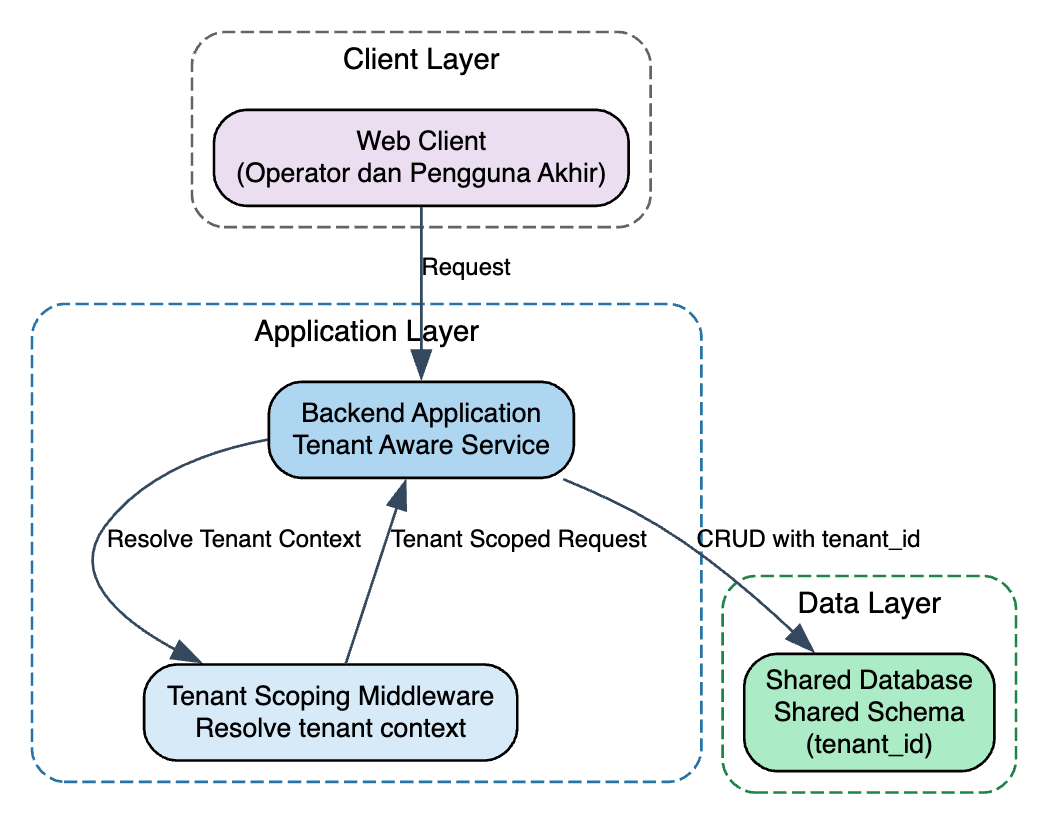
\includegraphics[width=0.9\textwidth]{assets/image3.png}
  \caption{Arsitektur Sistem Multitenant Berbasis \textit{Shared Database} dan \textit{Shared Schema}}
  \label{fig:arsitektur_multitenant}
\end{figure}

\section{Perancangan Model Penyimpanan Data}

Perancangan model penyimpanan data bertujuan untuk menjelaskan bagaimana pendekatan
\textit{shared database} dan \textit{shared schema} diterapkan pada sistem multitenant yang
dirancang. Model ini digunakan untuk mendukung efisiensi infrastruktur dengan tetap menjaga
isolasi data antar tenant melalui mekanisme pemisahan logis pada tingkat skema dan aplikasi.

\subsection{Struktur \textit{Shared Database}}

Sistem menggunakan satu basis data terpusat yang dipakai bersama oleh seluruh tenant. Seluruh
tabel disimpan dalam satu skema basis data yang sama, sehingga tidak terdapat pemisahan fisik
basis data atau skema untuk masing-masing tenant. Pendekatan ini dipilih untuk menyederhanakan
pengelolaan basis data, mengurangi duplikasi struktur data, serta mendukung proses
\textit{provisioning} tenant secara otomatis tanpa memerlukan pembuatan skema baru.

Struktur basis data dibagi menjadi dua kategori utama, yaitu tabel global dan tabel
\textit{tenant scoped}, yang masing-masing memiliki peran berbeda dalam mendukung arsitektur
multitenant.

\subsection{Peran \texttt{tenant\_id} dalam Isolasi Data}

Atribut \texttt{tenant\_id} berfungsi sebagai penanda utama untuk membedakan data milik
masing-masing tenant dalam tabel \textit{tenant scoped}. Setiap \textit{record} yang berkaitan
dengan data operasional organisasi, seperti aset, inventori, dan rental, selalu memiliki nilai
\texttt{tenant\_id} yang mengidentifikasi kepemilikan data tersebut.

Dalam setiap operasi basis data, \texttt{tenant\_id} disertakan secara implisit melalui mekanisme
\textit{tenant scoping} pada lapisan aplikasi. Dengan demikian, seluruh operasi baca dan tulis
data selalu dibatasi pada tenant yang sesuai, sehingga mencegah terjadinya akses data lintas
tenant meskipun seluruh data disimpan dalam satu skema yang sama.

\subsection{Pemisahan Tabel Global dan \textit{Tenant Scoped}}

Tabel global digunakan untuk menyimpan data yang bersifat umum dan tidak terikat pada tenant
tertentu, seperti data konfigurasi sistem global atau metadata yang berlaku untuk seluruh platform.
Tabel global tidak memiliki atribut \texttt{tenant\_id} karena datanya memang dimaksudkan untuk
digunakan bersama oleh seluruh tenant.

Sebaliknya, tabel \textit{tenant scoped} digunakan untuk menyimpan data yang bersifat spesifik
bagi masing-masing tenant. Seluruh tabel \textit{tenant scoped} wajib memiliki atribut
\texttt{tenant\_id} sebagai bagian dari kunci logis data. Pemisahan ini memastikan bahwa hanya
data yang relevan dengan konteks tenant yang dapat diakses dalam setiap operasi sistem.

\begin{figure}[h]
  \centering
  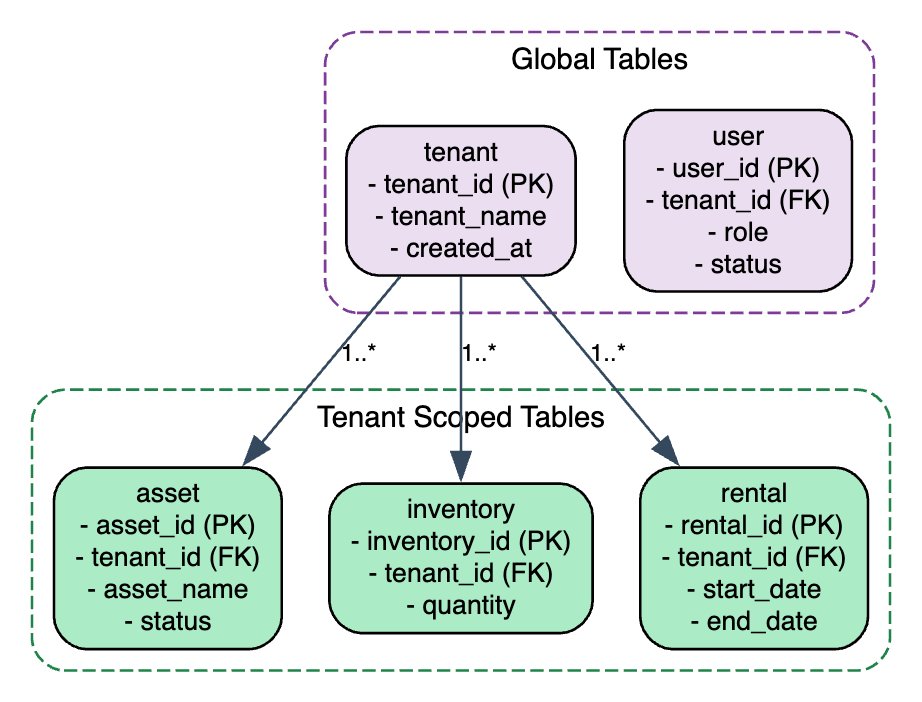
\includegraphics[width=0.9\textwidth]{assets/image4.png}
  \caption{Diagram Konseptual Model Penyimpanan Data \textit{Shared Schema}}
  \label{fig:model_penyimpanan}
\end{figure}

\section{Perancangan Mekanisme Isolasi Data}

Perancangan mekanisme isolasi data bertujuan untuk memastikan bahwa setiap tenant hanya dapat
mengakses data yang berada dalam konteks organisasinya masing-masing, meskipun seluruh tenant
berbagi aplikasi dan basis data yang sama. Pada arsitektur multitenant berbasis \textit{shared
database} dan \textit{shared schema}, isolasi data tidak dicapai melalui pemisahan fisik,
melainkan melalui mekanisme pengendalian konteks tenant pada lapisan aplikasi.

\subsection{\textit{Tenant Scoping} pada Lapisan Aplikasi}

\textit{Tenant scoping} merupakan mekanisme yang digunakan untuk menentukan dan mengelola konteks
tenant pada setiap permintaan yang masuk ke sistem. Dalam sistem yang dirancang, tenant tidak
ditentukan oleh pilihan pengguna secara manual, melainkan diidentifikasi secara otomatis oleh
sistem berdasarkan informasi yang dibawa pada permintaan, seperti token autentikasi atau metadata
permintaan.

Setelah tenant berhasil diidentifikasi, sistem menyimpan informasi \texttt{tenant\_id} ke dalam
konteks permintaan (\textit{request context}). Konteks ini kemudian digunakan secara konsisten
pada seluruh lapisan aplikasi, khususnya pada saat pembentukan \textit{query} basis data. Dengan
pendekatan ini, seluruh operasi data secara implisit dibatasi pada tenant yang sesuai tanpa
memerlukan intervensi pengguna.

\subsection{Alur \textit{Request Tenant Aware}}

Alur \textit{request tenant aware} dirancang agar setiap permintaan yang diproses oleh sistem
selalu berada dalam konteks tenant yang valid. Proses ini dimulai ketika pengguna mengirimkan
permintaan ke \textit{backend} melalui antarmuka web. Permintaan tersebut terlebih dahulu diproses
oleh komponen \textit{middleware tenant scoping} yang bertugas mengekstraksi identitas tenant dari
permintaan dan memverifikasinya.

Apabila identitas tenant valid, \textit{middleware} akan menambahkan \texttt{tenant\_id} ke dalam
konteks permintaan sebelum diteruskan ke lapisan layanan aplikasi. Layanan aplikasi kemudian
mengeksekusi logika bisnis dan operasi basis data dengan menyertakan \texttt{tenant\_id} sebagai
pembatas akses data. Alur \textit{tenant scoping} ini ditunjukkan pada Gambar \ref{fig:alur_tenant_scoping}.

\begin{figure}[h]
  \centering
  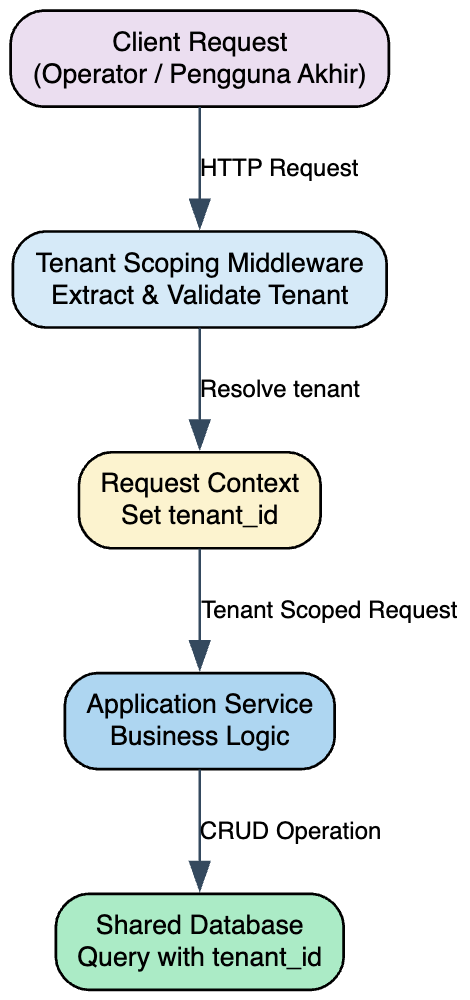
\includegraphics[width=0.45\textwidth]{assets/image5.png}
  \caption{Diagram Alur \textit{Tenant Scoping} pada Lapisan Aplikasi}
  \label{fig:alur_tenant_scoping}
\end{figure}

\subsection{Pembatasan Akses Data}

Pembatasan akses data diterapkan dengan memastikan bahwa setiap \textit{query} basis data terhadap
tabel \textit{tenant scoped} selalu menyertakan kondisi berdasarkan \texttt{tenant\_id}. Pendekatan
ini mencegah kemungkinan akses lintas tenant, baik secara sengaja maupun tidak sengaja. Dengan
menjadikan \texttt{tenant\_id} sebagai bagian wajib dalam seluruh operasi data, sistem dapat
menjamin bahwa data yang diambil atau dimodifikasi selalu sesuai dengan konteks tenant yang aktif.

Selain itu, pembatasan akses juga didukung oleh pengaturan hak akses berbasis peran pada tingkat
aplikasi, sehingga pengguna hanya dapat melakukan operasi yang sesuai dengan perannya dalam
konteks tenant masing-masing. Kombinasi antara \textit{tenant scoping} dan kontrol akses berbasis
peran membentuk mekanisme isolasi data yang konsisten dan terkontrol.

\section{Perancangan Proses \textit{Provisioning} Tenant}

Perancangan proses \textit{provisioning} tenant bertujuan untuk memastikan bahwa penambahan tenant
baru pada sistem multitenant dapat dilakukan secara otomatis, konsisten, dan efisien tanpa
memerlukan konfigurasi manual tambahan. Pada platform multi organisasi berskala nasional, proses
\textit{onboarding} tenant yang tidak terstandarisasi akan meningkatkan kompleksitas operasional
dan berpotensi menimbulkan ketidakkonsistenan konfigurasi sistem.

\subsection{Alur \textit{Provisioning} Tenant Otomatis}

\textit{Provisioning} tenant pada sistem yang dirancang dilakukan sepenuhnya oleh sistem di sisi
\textit{server}. Proses ini dipicu ketika terdapat permintaan pendaftaran organisasi baru atau
inisialisasi tenant melalui mekanisme yang telah ditentukan oleh platform. Sistem kemudian
menjalankan serangkaian langkah terstruktur untuk membentuk tenant baru tanpa keterlibatan aktor
administrator khusus.

Alur \textit{provisioning} dimulai dengan validasi data awal tenant, dilanjutkan dengan pembuatan
identitas tenant pada tabel global, serta inisialisasi konfigurasi standar yang berlaku untuk
seluruh tenant. Setelah proses ini selesai, tenant dinyatakan aktif dan siap digunakan oleh
pengguna operasional. Alur \textit{provisioning} tenant otomatis ini ditunjukkan pada Gambar \ref{fig:provisioning_tenant}.

\begin{figure}[h]
  \centering
  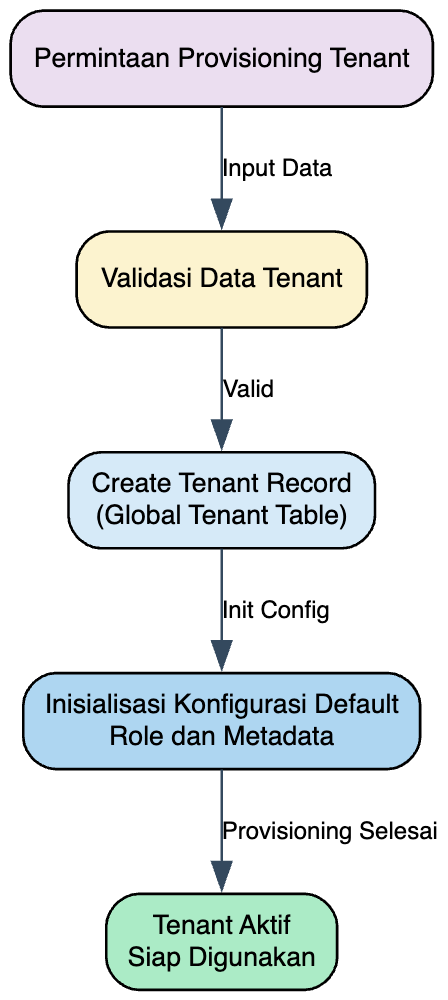
\includegraphics[width=0.45\textwidth]{assets/image6.png}
  \caption{Diagram Proses \textit{Provisioning} Tenant Otomatis}
  \label{fig:provisioning_tenant}
\end{figure}

\subsection{Data dan Konfigurasi yang Diinisialisasi}

Pada saat \textit{provisioning} tenant dilakukan, sistem menginisialisasi sejumlah data dan
konfigurasi dasar agar tenant dapat langsung beroperasi. Data dan konfigurasi tersebut meliputi
identitas tenant, struktur akses dasar, serta metadata yang diperlukan untuk pengelolaan konteks
tenant pada lapisan aplikasi. Seluruh data yang diinisialisasi mengikuti standar yang sama untuk
setiap tenant, sehingga tidak terjadi perbedaan konfigurasi antar tenant yang disebabkan oleh
intervensi manual.

Pendekatan ini memastikan bahwa setiap tenant memiliki struktur data dan konfigurasi awal yang
konsisten, serta dapat langsung menggunakan sistem tanpa memerlukan penyesuaian tambahan pada
tingkat aplikasi maupun basis data.

\subsection{Perbandingan \textit{Provisioning} Manual dan Otomatis}

Pada pendekatan \textit{provisioning} manual, penambahan tenant baru biasanya memerlukan pembuatan
konfigurasi sistem secara terpisah, termasuk penyesuaian basis data, pengaturan akses, dan
validasi konfigurasi. Pendekatan ini tidak efisien dan berisiko menimbulkan kesalahan konfigurasi,
terutama ketika jumlah tenant meningkat.

Sebaliknya, \textit{provisioning} tenant otomatis pada arsitektur multitenant berbasis
\textit{shared database} dan \textit{shared schema} memungkinkan penambahan tenant baru tanpa
perubahan struktur sistem. Seluruh proses dilakukan oleh sistem berdasarkan alur yang telah
ditentukan, sehingga mengurangi beban operasional dan meningkatkan konsistensi konfigurasi.

\section{Rancangan Evaluasi dan Parameter Pengujian}

Rancangan evaluasi disusun untuk memastikan bahwa arsitektur multitenant yang dirancang
benar-benar memenuhi tujuan penelitian serta mampu menjawab permasalahan yang telah dirumuskan.
Evaluasi tidak difokuskan pada pengukuran performa sistem secara kuantitatif tingkat rendah,
melainkan pada kesesuaian rancangan arsitektur terhadap aspek efisiensi infrastruktur, isolasi
data antar tenant, dan efektivitas \textit{provisioning} tenant otomatis.

\subsection{Parameter Evaluasi Efisiensi Infrastruktur}

Efisiensi infrastruktur dievaluasi dengan meninjau sejauh mana arsitektur multitenant berbasis
\textit{shared database} dan \textit{shared schema} mampu mengurangi kebutuhan sumber daya sistem
dibandingkan pendekatan non multitenant. Parameter evaluasi difokuskan pada kompleksitas
konfigurasi sistem dan dependensi infrastruktur yang diperlukan untuk mendukung banyak tenant
dalam satu platform.

Parameter yang digunakan antara lain jumlah konfigurasi sistem yang harus dikelola, jumlah
komponen infrastruktur yang dibutuhkan, serta kebutuhan penyesuaian konfigurasi ketika tenant
baru ditambahkan. Arsitektur dinilai efisien apabila penambahan tenant tidak memerlukan penambahan
\textit{instance} aplikasi atau basis data baru.

\subsection{Parameter Evaluasi Isolasi Data Antar Tenant}

Evaluasi isolasi data bertujuan memastikan bahwa mekanisme \textit{tenant scoping} dan penggunaan
\texttt{tenant\_id} mampu mencegah akses data lintas tenant. Parameter evaluasi difokuskan pada
konsistensi pembatasan data pada setiap operasi basis data dan kemampuan sistem menolak atau
membatasi akses yang berada di luar konteks tenant.

Pengujian dilakukan melalui simulasi permintaan dari tenant yang berbeda untuk memastikan bahwa
data yang dikembalikan oleh sistem selalu sesuai dengan tenant yang aktif. Isolasi data dinyatakan
terpenuhi apabila tidak ditemukan data milik tenant lain pada hasil pengujian.

\subsection{Parameter Evaluasi \textit{Provisioning} Tenant Otomatis}

Evaluasi \textit{provisioning} tenant dilakukan untuk menilai efektivitas proses
\textit{onboarding} tenant tanpa konfigurasi manual tambahan. Parameter evaluasi difokuskan pada
konsistensi konfigurasi tenant baru, keseragaman struktur data awal, serta kemampuan tenant untuk
langsung menggunakan sistem setelah proses \textit{provisioning} selesai.

\textit{Provisioning} tenant dinyatakan berhasil apabila setiap tenant baru memiliki konfigurasi
awal yang identik dan tidak memerlukan penyesuaian tambahan pada tingkat aplikasi maupun basis
data.
